%%% The main file. It contains definitions of basic parameters and includes all other parts.


%% Settings for two-sided (duplex) printing
\documentclass[10pt,a4paper]{report}
\let\openright=\cleardoublepage

%% Character encoding: usually latin2, cp1250 or utf8:
\usepackage[utf8]{inputenc}

%% It's 2019
\usepackage[default]{droidserif}
\usepackage[T1]{fontenc}

%% Further useful packages (included in most LaTeX distributions)
\usepackage{amsmath}        % extensions for typesetting of math
\usepackage{amsfonts}       % math fonts
\usepackage{graphicx}       % embedding of pictures
\usepackage{tikz}
%\usetikzlibrary{shapes,fit,positioning,snakes,mindmap,trees,decorations.text,arrows.meta}
%\makenomenclature
\usepackage{algorithm,algpseudocode}
\usepackage{booktabs}
\usepackage{mwe}
\usepackage{pgfgantt}
\usepackage{pdflscape}
\usepackage{geometry}
\usepackage{enumitem}
\usepackage{float}
\usepackage{framed}
\usepackage{titlesec}
\usepackage{listings}
\lstset{basicstyle=\ttfamily,
	showstringspaces=false,
	commentstyle=\color{red},
	keywordstyle=\color{blue}
}

\usepackage{pdfpages}

\usepackage[textsize=tiny,backgroundcolor=yellow!50, linecolor=black!25]{todonotes}

% links shall be clickable
\usepackage[unicode]{hyperref}   % Must follow all other packages
\usepackage{cleveref} % Must follow all other packages including hyperref

% Definitions of macros (see description inside)

\newcommand{\cool}{\color{green!50!white!80!black}}
\newcommand{\textcool}[1]{{\cool #1}}

\newcommand{\XX}[1]{\textcolor{red}{#1}}
\newcommand{\TT}[1]{\texttt{#1}}
\newcommand{\X}[1]{\textsc{#1}}

% Draw black "slugs" whenever a line overflows, so that we can spot it easily.
% TODO remove this later, no one actually cares for spec purposes
\overfullrule=1mm

% avoid some slugs naturally
\clubpenalty=1000
\widowpenalty=1000
%\hyphenpenalty=100  % turn this on to prevent hyphenation
\emergencystretch=2cm


%%% The field of all real and natural numbers
\newcommand{\R}{\mathbb{R}}
\newcommand{\N}{\mathbb{N}}
\newcommand{\F}{\mathbb{F}}
\newcommand{\Z}{\mathbb{Z}}

\newcommand{\bms}{\begin{enumerate}[label=\bf (M\arabic*)]}
\newcommand{\bwp}{\begin{enumerate}[label=\bf \normalsize  (WP\arabic*), resume=del]}
\newcommand{\eenum}{\end{enumerate}}
\newcommand{\itemm}{\large \item }
\newcommand{\itemwp}{ \normalsize \item }
\newcommand{\deadline}[1]{\textit{\small (month #1)}}
\newcommand{\people}[1]{\textit{\small (#1)}}


% move the headings out of gutenberg era
\setcounter{secnumdepth}{4}
\titleformat{\chapter}{\cool\fontsize{24pt}{24pt}\bfseries}{\color{black!25}\thechapter.}{1em}{}
\titleformat{\section}{\cool\fontsize{16pt}{18pt}\bfseries}{\scriptsize\color{black!25}\thesection}{1em}{}
\titleformat{\subsection}{\cool\fontsize{14pt}{16pt}\bfseries}{\scriptsize\color{black!25}\thesubsection}{1em}{}
\titleformat{\subsubsection}{\cool\fontsize{12pt}{14pt}\bfseries}{\scriptsize\color{black!25}\thesubsubsection}{1em}{}



\title{\textcool{\bf High Level Assembler Plugin} \\ Project specification}
\author{Michal Bali, Marcel Hruška, Peter Polák,\\ Adam Šmelko, Lucia Tódová}
\date{Supervisor: Miroslav Kratochvíl}

% Title page and various mandatory informational pages
\begin{document}
\maketitle

%%% A page with automatically generated table of contents of the bachelor thesis

\tableofcontents

%%% Each chapter is kept in a separate file
\chapter*{Introduction}
\addcontentsline{toc}{chapter}{Introduction}
\cite{CoDel}

\section*{Related Work}


\chapter{HLASM overview}

Assembly languages consist of solely ordinary machine instructions. High-level assemblers generally extend them with features commonly found in high-level programming languages, such as control statements similar to \emph{if, while, for} as well as custom callable macros.

IBM High Level Assembler (HLASM) satisfies this definition and adds other features which will be described in this chapter.

\section{Syntax}

Due to historical reasons, HLASM syntax differs greatly to the syntax of modern programming languages. It mostly uses syntax common to regular assemblers, which has limitations, like line-length limited to 80 characters (as that was the length of a punched card line).

\subsection{Statement}

HLASM program is represented by a sequence of \emph{statements}. A statement consists of four fields. These are:
\begin{itemize}
	\item \textbf{Name field} --- Serves as a place for named constants that are to be used in code. This field is optional, but, when present, it must start at the begin column of a line.
	
	\item \textbf{Operation field} --- The only mandatory field representing the instruction that is executed. Must not begin in the first column, as it would be interpreted as a name field.
	
	\item \textbf{Operands field} --- Field for instruction operands, located immediately after operation field. Individual operands must be separated by a comma, and, depending on the specific instruction, can be either blank, in a form of an apostrophe separated string, or represented by a sequence of characters.
	
	\item \textbf{Remark field} --- Optional, serves as inline commentary. Located either after the operands field, or, in case the operands are omitted, the operation field. 
\end{itemize}


\Cref{lst:small_example} shows an example of a basic statement containing all fields.
\begin{listing}

\begin{verbatim}
 label   instruction     operands             remarks
.NOMOV       AGO     (&WH).L1,.L2,.L3     SEQUENTIAL BRANCH
\end{verbatim}
\caption{An example statement with fields.}
\label{lst:small_example}
\end{listing}

\subsection{Continuation}

Individual statements sometimes contain more than 80 characters, which contradicts to line length limitations. Therefore, a special handling called \emph{continuation} is introduced.

Firstly, let us elaborate more on the topic of line columns. There are four special columns:
\begin{itemize}
	\item \emph{Begin column (default value: 1)}
	
	\item \emph{End column (default value: 71)}
	
	\item \emph{Continuation column (default value: 72)}
	
	\item \emph{Continue column (default value: 16)}
\end{itemize}
They all serve a different purpose.

\emph{Begin column} defines either the start of a statement, or the beginning of the name field.

\emph{End column} determines the end of the statement. Anything written to its right does not count as content of the statement, and is rather used as a place for the line sequence number (see \cref{fig01:line}). 

\emph{Continuation column} is used to indicate that the statement continues on the next line. For proper indication, an arbitrary character other than space must be written in this column. The remainder of the statement must then start on the \emph{continue column}.

An example of an instruction where its last operand exceeded 72.~column of the line can be seen in \cref{lst:overflow}.
\begin{listing}
	\begin{verbatim}
             OP1                   REG12,REG07,REG04,REG00,REG01,REG11,Rx
                EG02
	\end{verbatim}
	\caption{Example program that uses continuation for overflowing the line.}
	\label{lst:overflow}
\end{listing}

There also exist instructions that support a so called \emph{extended format} of the operands. It allows the presence of a continuation character even when the contents of a line have not reached the continuation column (see \cref{lst:extended}).

\begin{listing}
\begin{verbatim}
          AIF   ('&VAR' FIND '~').A,     REMARK1                        x
                ('&VAR'  EQ  'L').B,     REMARK2                        x
                (T'&VAR  EQ  'U').C      REMARK3 
\end{verbatim}
\caption{Extended instruction format.}
\label{lst:extended}
\end{listing}

\begin{figure}
	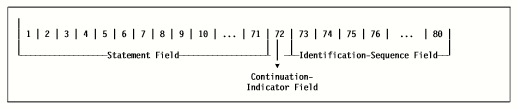
\includegraphics[width=\textwidth]{img/line}
	\caption{Description of line columns (source: \href{https://www-01.ibm.com/servers/resourcelink/svc00100.nsf/pages/zOSV2R3sc264940/$file/asmr1023.pdf}{HLASM Language Reference} ).}
	\label{fig01:line}
\end{figure}


\section{Assembling}

Having briefly described its syntax, this section prepares the reader to better understand the assembly process hidden behind HLASM. 

HLASM program consists of sequence of statements. Those statements are mainly ordinary \emph{machine instructions} that are processed and tranlated into corresponding opcodes. This does not differ from traditional assemblers.

In addition to machine instruction statements, HLASM assembler provides the \emph{assembler instructions} (in other systems commonly termed as \emph{directives}). They order the assembler to take a specific actions rather than assembling instructions. For example, they generate run-time data constants, create named symbols containing relative addresses or constant values, modify addresses of code generation or affect how the assembler operates.

On top of this, the HLASM assembler offers \emph{conditional assembly (CA) processing}. The user may think of it as a macro-language built above traditional assembler. Employing special statements, user is capable of branching around and printing machine instruction statements. Even more, the user is able to define custom macros that can be called defined with parameters. Note, that CA processing is T-complete and it is whole processed during compile-time.

The last think to note is that CA processing, although it may act like a text preprocessing, is still interlinked with ordinary processing. CA have mechanics that allow user to gather information about statements that are printed during the processing.

\vspace{5mm}

Now, let us talk more about above described kinds of processing.

\subsection{Conditional assembly}

Conditional assembly processing can be divided into \emph{variable symbols}, \emph{conditional assembly instructions} and \emph{macros}. 

\subsubsection{Variable symbols}

Variable symbols serve as points of substitution or information holders. 

When they occur in a statement, they are substituted by their value to create a new statement. For example, in this manner, a user can write a variable symbol in an operation field of a statement and generate any instruction that can be a result of a substitution.

Variable symbols also have notion of their type --- they can be defined either as an integer, a boolean or a string. CA instructions gather this information for different sorts of conditional branching.

\subsubsection{CA instructions}

The major difference to other instructions is that they are not assembled into object code. Rather, they select which instructions will be processed by assembler next.

One subset of CA instructions operates on variable symbols. With them, the user can define variable symbols locally or globally, assign or update their values.

Other subset is capable of conditional and unconditional branching. HLASM provides a variety of built-in binary or unary operations on variable symbols, which can create complex conditional expressions. This is important in HLASM, as the user can alter flow of instructions that will be assembled into executable program.

\subsubsection{Macros}

A \emph{macro} is a structure consisting of a \emph{name}, \emph{input parameters} and a \emph{body}, which is a sequence of statements. When a macro is called in a HLASM program, each statement in its body is executed. Both nested and recursive calls of macros are allowed. Macro body can contain CA instructions or even a sequence of instructions generating another macro definition.

With the help of variable symbols, HLASM macros have the power to create custom, task specific macros.

\subsection{Assembler instructions}
Here, let us enumerate a few of the assembler instructions:
\begin{itemize}
	\item \textbf{ICTL} --- Changes values of the previously described line columns (i.e. begin column may begin at column 2 etc.).
	
	\item \textbf{DC} --- Reserves space in object code for data described in operands field and assembles them in place (i.e. assembles float, double, character array, address etc. ).
	
	\item \textbf{EQU} --- Defines named constant with an integer or a relative address value. These constants can be accessed by \emph{conditional assembly}, hence alter it in custom manner.
	
	\item \textbf{COPY} --- Copies a whole file found in \emph{copy member library}\footnote{Path to library is passed to assembler before the start of assembly} and pastes it in place of the instruction.
	
	\item \textbf{CSECT} --- Creates an executable control section. Serves as the beginning of a machine instruction sequence and as the start of relative addressing.
\end{itemize}

\subsection{Machine instructions}
\emph{Machine instructions} and their operands are translated to a sequence of bytes and written to the executable program. In contrast to basic assemblers, HLASM allows expressions to be passed as operands of these instructions. These expressions are capable of address arithmetics, and can also contain defined constants.

\vspace{5mm}

An example of simple HLASM program with the description of its statements is shown in \cref{lst:example}.
\begin{listing}
\begin{verbatim}
         name        operation   operands
         
[01]                 MACRO                   
[02]     &NAME       GEN_LABEL
[03]     &NAME       EQU         *
[04]                 MEND
[05]             
[06]                 COPY        REGS
[07]             
[08]     TEST        CSECT
[09]     &VAR        SETA        L'DOUBLE
[10]                 AIF         (&VAR EQ 4).END
[11]     LBL1        GEN_LABEL
[12]                 LR          3,2
[13]                 L           8
[14]     LBL2        GEN_LABEL
[15]     LEN         EQU         LBL2-LBL1
[16]                 DC          (LEN)C'HELLO'
[17]     DOUBLE      DC          D'-3.729'
[18]     .END        ANOP
[19]                 END
\end{verbatim} 
\caption{An example of HLASM program.}
\label{lst:example}
\end{listing}

In lines \verb|01-04|, we see a \emph{macro definition}. It is defined with a name \verb|GEN_LABEL|, variable \verb|NAME| and contains one instruction in its body, which assigns the current address to the label in \verb|NAME|.

In line \verb|06|, the \emph{copy instruction} is used, which includes the contents of the \verb|REGS| file.

Line \verb|08| establishes a start of an executable section \verb|TEST|. 

In line \verb|09|, an integer value is assigned to a variable symbol \verb|VAR|. The value is the length attribute of previously non-defined constant \verb|DOUBLE|. The assembler looks for the definition of the constant to properly evaluate the conditional assembly expression. In the next line, there is CA branching instruction \verb|AIF|. If value of \verb|VAR| equals to 4, next lines are skipped and assembling continues on line \verb|18|, where branching symbol \verb|END| is located.  

Lines \verb|12-13| show examples of machine instructions that are directly assembled into object code. Lines \verb|11,14| contain examples of macro call.

In line \verb|15|, the constant \verb|LEN| is assigned the difference of two addresses. This value is next used to generate character data.

Instruction \verb|DC| in line \verb|17| creates value of type double and assigns its address to constant \verb|DOUBLE|. This constant also holds information about length, type and other attributes of the data.  

\verb|ANOP| is an empty assembler action and line \verb|19| ends the assembling of the program. 
\chapter{Project scope}

This chapter reviews the specific goals of our project.
All the features below have been discussed with professional HLASM developers and have been agreed on by the company.

This project aims to produce a VS Code extension, downloadable from the Market Place. The extension contains all executables/libraries that are needed for the project to work correctly on the most popular platforms. No other prerequisites should be needed.

Modularity of the software is another important requirement. 

The parsing library provides 2 kinds of API: a complex one that mirrors the LSP specification and a simple one that accepts a text along with a dependency-resolver object and returns diagnostics. 

The language server implements the LSP standard, hence it can be easily reintegrated within other IDEs such as Eclipse Che.

\section{Supported language features}
This part provides a brief overview of the parts of HLASM that should be included in the final software.

\begin{itemize}
\item The parsing library recognizes the syntax of HLASM and parses it into predefined structures. 

\item It is able to interpret high-level parts of the assembler. Following are the conditional assembly instructions for code generation and macro expansion:
\begin{itemize}
    \item AIF
    \item AGO
    \item MACRO, MEND, MEXIT
    \item ACTR
    \item SETA, SETB, SETC
    \item ANOP
    \item LCLA, LCLB, LCLC
    \item GBLA, GBLB, GBLC
    \item AEJECT
    \item ASPACE
\end{itemize}
and assembler instructions for code layout determination:
\begin{itemize}
    \item EQU 
    \item DC 
    \item DS 
    \item DSECT, CSECT, RSECT 
    \item LOCTR
\end{itemize}

\item The back-end library also semantically and syntactically checks all instructions (including machine instructions) for correct operand format usage. However, it does not analyze the run-time register and memory values, as there is no machine instruction interpretation.

\item Usage of external files in HLASM is a highly common phenomenon. On mainframes, HLASM programs are built according to its JCL\footnote{Job Control Language, instructs the system how to run a specific task} file, which contains a list of libraries. When the compiler encounters an undefined instruction or a \texttt{COPY} instruction, it does a top-down search through the whole list. Both ways of invoking a dependency search are demonstrated in \cref{lst:search}. As a large portion of the programs use the same libraries, defining these JCL files gets repetitive. Therefore, the build and source management system Endevor creates an abstraction above the libraries and groups them into \texttt{processor groups}. As a result, JCL offers an option to identify the libraries to be included by their processor group's ID instead of listing them all manually.

We adapt this system to our needs and define 2 configuration files. The first one mirrors the behavior of Endevor and defines the processor groups. The second one matches the source codes to these processor groups.

\item Another aspect of HLASM that needs to be considered and handled are fixed-sized lines. This makes the parsing more difficult, as the position of the continuation character may vary. We also add a continuation handling option to the IDE, which mostly consists of non-movable continuation characters, i.e. if the user types something in front of the continuation character, it stays on place.

\item On top of that, we implement the \texttt{macro tracer} using the \texttt{Debug Adapter Protocol}. Following the standard debugging procedure, the user can step through the code generation while watching the contents of variables and the call stack. This tool is extremely useful as tracing the macro expansions manually gets tedious quickly.
\end{itemize}

\pagebreak
\begin{listing}
\begin{verbatim}
        MAC1       1,1                   
        COPY       COPY1
\end{verbatim} 
\caption{An example of both ways the HLASM program may invoke dependency search.}
\label{lst:search}
\end{listing}

\section{Supported LSP features}
This section demonstrates the possible uses of the extension on the client side. LSP provides a list of well-defined features. The project implements the following:

\begin{itemize}
	\item \texttt{Go to definition} command for all symbols, macro definitions and copy members\footnote{Copy, along with macro expansion, is a mean to include another external file, invoked by \texttt{COPY} instruction. Comparing to macro, copy does not neither need to start nor end with any specific instruction and the invoking \texttt{COPY} instruction is simply replaced by the COPY file's contents.}
	\item \texttt{Find all references} command for all symbols, macro definitions and copy members
	\item Completion for instructions, defined symbols and macros
	\item Hover for symbol attributes, their locations, contents and other useful information depending on the symbol type
	\item Diagnostics for syntax and semantic errors and warnings
	\item (Custom LSP extension) Server-side Highlighting for all symbols  
\end{itemize}

The highlighting is not a standard part of the LSP, nonetheless it is a needed addition. Due to the complexity of HLASM, a typical syntax highlighting is not sufficient. Consider following examples:

\lstdefinelanguage{HLASM}{
    keywords = [1]{REMARK},
    keywords = [2]{SAM31,LR,AGO,AIF,ICTL},
    keywords = [3]{J,SYMBOL},
     keywords = [4]{IGNORED},
     keywords = [5]{X},
    keywordstyle = [1]\color{blue},
    keywordstyle = [2]\color{red},
    keywordstyle = [3]\color{white},
    keywordstyle = [4]\color{magenta},
    keywordstyle = [5]\color{cyan}
}
\lstset{
numbers=left, 
numberstyle=\small, 
numbersep=8pt, 
frame = single, 
language=HLASM, 
framexleftmargin=15pt,
backgroundcolor = \color{lightgray}
}
\begin{itemize}
    \item The language server recognizes operand formats of different instructions. The most simple example is the \texttt{SAM31} instruction, which does not have any operands, while the \texttt{LR} instruction takes two. So the identifier right after \texttt{SAM31} is colored blue as a remark. 
    
\begin{lstlisting}
    SAM31 REMARK
    LR    1,1   REMARK
\end{lstlisting}

\item The code skipped by the conditional assembly is not colored and stays white.
\begin{lstlisting}
    AGO .HERE
    J   SYMBOL
.HERE AIF
\end{lstlisting}

\end{itemize}


\chapter{Architecture}

\todo{Nedohodli sme sa na americkej anglictine?}

\begin{figure}
	\centering
	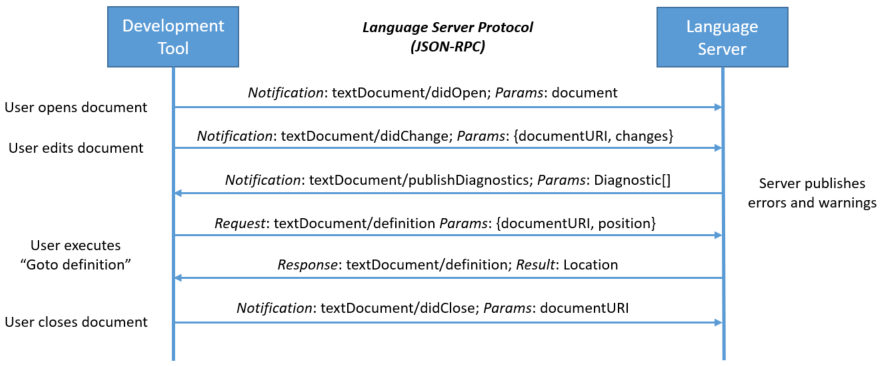
\includegraphics[width=\textwidth]{img/language-server-sequence}
	\caption{LSP session example }
	\label{fig04:LSP}
\end{figure}\todo{nechyba zdroj (Adam to daval, tak aby sme boli konzistentni) \ref{fig04:LSP}?}

\begin{figure}
	\centering
	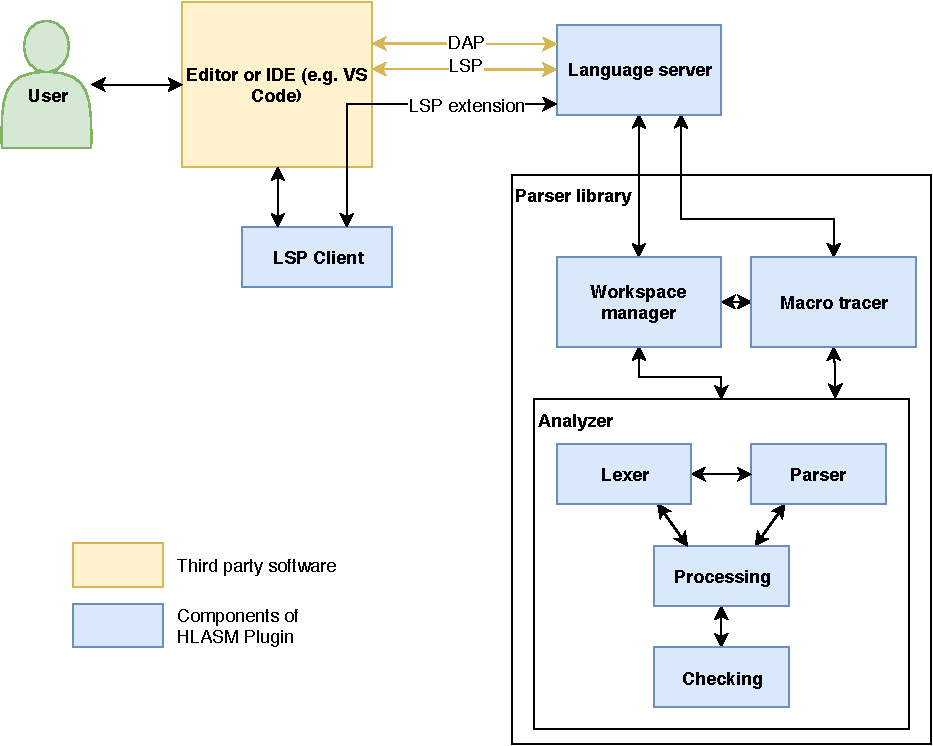
\includegraphics[width=\textwidth]{img/hlasm_architecture}
	\caption{The architecture of HLASM Plugin}
	\label{fig04:arch}
\end{figure}



The architecture is based on the way modern code editors and IDEs are extended to support additional languages. We chose to implement Language Server Protocol \footnote{https://microsoft.github.io/language-server-protocol/} (LSP), which is supported by a majority of contemporary editors.

In LSP, the two parties that communicate are called a \emph{client} and a\emph{language server}. A simple example is displayed in Figure~\cref{fig04:LSP} The client runs as a part of an editor. The language server may be a standalone application that is connected to the client by a pipe or TCP. All language-specific user actions are transformed into standard LSP messages and sent to the language server. The language server then analyzes the source code and sends back a response, which is then interpreted and presented to the user in editor-specific way. This architecture makes possible to only have one LSP client implementation for each code editor, which may be reused by all programming languages. And vice versa, every language server may be easily used by any editor that has an implementation of the LSP client.
\todo{mozno pridat editory: Eclipse, Vim, IntelliJ... }

To add support for HLASM, we have to implement the LSP language server and write a thin extension to an editor, which will use an already existing implementation of the LSP client. To implement source code highlighting, we need to extend the protocol with a new notification. This notification will be used for transferring information from language server to VS Code client, which is extended to highlight code in editor based on the incoming custom notifications.

This chapter presents the decomposition of the project into smaller components and describes their relations. The two main components are the parser library and the language server --- an executable application that uses the parser library. The overall architecture is pictured in Figure~\cref{fig04:arch}.

\section{Language server}

The responsibility of the Language server component is to maintain the LSP session, convert incoming JSON messages and use the parser library to execute them. The functionality includes:
\begin{itemize}
    \item reading LSP messages from standard input or TCP and writing responses
    \item parsing JSON RPC to C++ structures, so they can be further used
    \item serializing C++ structures into JSON, so it can be sent back to the client
    \item implementing asynchronous request handling: e.g. when user makes several consecutive changes to a source code, it is not needed to parse on every change
\end{itemize}

\section{Parser library}

Parser library is the core of the project --- it encapsulates all parsing capabilities, keeps track of open files in the editor and provides information about them. Its API is based on LSP --- every relevant request and notification has a corresponding method in the parsing library. The API includes:

\begin{itemize}
	\item Implementation of text synchronization notifications (didOpen, didChange, didClose), which inform the library about files that are currently open in the editor and their exact contents.
	\item Implementation of workspace management notifications (DidChangeWorkspaceFolders): many editors have \todo[inline]{capability mozno lepsie} possibilities to open more workspaces at the same time, and the parser library supports this too. Workspace is basically just a folder which contains related source codes. Workspaces help parser library find macro and copy files.
	\item A method to consume DidChangeWatchedFiles notification. This method makes it possible to react to workspace changes that were not made by the user in editor, but may still affect the parsing. For example, when a user deletes an external macro file, the parser library should react by reporting that it cannot find the macro.
	\item Implementation of diagnostics publishing (publishDiagnostics notification). A diagnostic is used to indicate a problem with source files, such as a compiler error or a warning. The parser library provides a callback to let the language server know that diagnostics have changed.
	\item Callback for highlighting information provision.
	\item Implementation of language feature requests (definition, references, hover, completion), which provide information needed for proper reaction of the editor on user actions.
	
\end{itemize}

The parser library is further decomposed into smaller components.

\subsection{Analyzer}

The analyzer is able to process a single HLASM file. The processing includes:
\begin{itemize}
 \item recognition of statements and their parts (lexing and parsing)
 \item interpretation of instructions that should be executed in compile time
 \item a check whether the HLASM source code is well-formed
 \item reporting of problems with the source by producing LSP diagnostics
 \item providing highlighting and LSP information
\end{itemize}

A HLASM file may have dependencies --- other files that define macros or files brought in by the COPY instruction. The dependencies are only discovered during the processing of files, so it is not possible to provide the files beforehand. The analyzer must get a callback that would find a file with specified name, parse its contents and return it as list of parsed statements. 

To sum up, the analyzer has a pretty simple API: it takes the contents of a source file by common string and a callback that can parse external files with specified name. It provides a list of diagnostics linked to the file, highlighting, list of symbol definitions, etc.

The analyzer is further decomposed into 4 components.

\subsubsection{Lexer}

Lexer's task is to read source string and break it into tokens --- small pieces of text with special meaning. The most important properties of the lexer:
\begin{itemize}
	\item each token has location in the source text
	\item has the ability to check whether all characters are valid in the HLASM source
	\item has the ability to jump in the source file backward and forward if necessary (for implementation of instructions like AGO and AIF)
\end{itemize}

\todo{Because of the complexity and specificity of HLASM language we implement our own lexer from scratch even though there are many tools for lexical analysis.}

\subsubsection{Parser}

Parser component takes the stream of tokens the lexer produces and recognizes HLASM statements according to syntax. To accomplish this, a parser generator tool Antlr 4 \footnote{https://www.antlr.org} is used.

The input to Antlr is a grammar (written in antlr-specific language) that specifies the syntax of HLASM language and generates source code (in C++) for a recognizer, which is able to tell whether input source code is valid or not. Moreover, it is possible to assign a piece of code that executes every time a grammar rule is matched by the recognizer to further process the matched piece of code.


\subsubsection{Processing}

Results of the parser component are further analyzed in the processing component. Its most important capabilities are:
\begin{itemize}
	\item Interpretation of CA instructions, which results in modifying the lexer state (moving back and forth in the input file).
	\item Substitution of variable symbols. After the substitution, the statement must be reparsed in the lexer and the parser.
	\item Interpretation of assembler instructions to evaluate ordinary symbols.
	\item MACRO and COPY expansion.
\end{itemize}

\subsubsection{Checking}
After a statement is fully processed and all operands of each instruction are known, the statement needs to be checked for errors. There are over 2000 machine instructions with variable number of operands and various restrictions on those operands --- some of them take only positive numbers, numbers that are in specific range or are limited to addresses only. The checking component takes an instruction and list of its operands and returns a list of warnings or error in a form of LSP diagnostics.

\subsection{Workspace manager}

The responsibility of a workspace manager is to keep the representation of workspaces and files in the parser library exactly the same as the user sees in the editor. Further, it starts the analyzer when needed, manages workspace configuration and provides external macro and copy libraries to analyzer.

\section{VS code extension}

The VS Code extension component ensures seamless integration with the editor. Its functions are:

\begin{itemize}
	\item to start the HLASM language server and the LSP client that comes with VS Code, and create a connection between them
	\item to implement server-side highlighting, which extends the LSP protocol
	\item to improve user experience regarding continuations and fixed length line source codes
\end{itemize}


\section{Macro tracer}
A macro tracer enables the user to trace the compilation of HLASM source code in a way similar to common debugging. This is the reason why we chose to implement a Debug Adapter Protocol \footnote{https://microsoft.github.io/debug-adapter-protocol/} (DAP). It is very similar to LSP, so most of the code implementing LSP in the language server component may be reused for both protocols.

The language server component communicates with the macro tracer component in the parser library. Its API mirrors the requests and events of DAP. The most important features to implement are:

\begin{itemize}
	\item launch, continue, next, stepIn and disconnect requests, which allow user to control the flow of the compilation
	\item SetBreakpoints, which get information about breakpoints that the user has placed in the code
	\item Threads, StackTrace, Scopes and Variables requests to allow the DAP client to retrieve information about the current processing stack (stack of nested macros and copy instructions), available variable symbols and their values
	\item stopped, exited and terminated events to let the DAP client know about state of traced source code
\end{itemize}

The macro tracer communicates with the workspace manager to retrieve the content of the traced files. Afterwards, it starts analyzing the source file in a separate thread and gets callbacks from the analyzer before a statement is processed. In the callback, the tracer puts the thread to sleep and waits for user interaction. During this time, it is possible to retrieve all variable and stack information from the processing to display it to the user.

%probably not needed?
%\chapter{Technologies}

\todo{tohle patri do Architecture, pripadne to prejmenujte na `Implementation details' nebo tak cosi.}
mirko: soupis konkretnich technologii a verzi
antlr
cmake
jenkins
json lib
boost asio?
docker

vscode 
theia
che
produkcne zdrojaky poskytnute broadcom
google test

--jenkins sa opytat ako s tym ze to nie je nase

jazyky
typescript 
c++
cmake

\chapter{Project execution}

In the following chapter is represented execution of the High Level Assembler Plugin software project. 
We analyze the problem difficulty, break it into tasks and estimate time requirements of particular tasks.
We further describe the team and work organization.

\section{Tasks}
We analyzed the problem and split it into several tasks. These were assigned to individual team members. The tasks and their assignment (team member name initials in the parentheses following task name) is summarized in the Gantt diagram(s)  (\ref{fig:gantt1}, \ref{fig:gantt2}, \ref{fig:gantt3}). 
Project implementation is planned for nine months. At the time of writing implementation is already in the 24. week of our schedule.	

\section{Collaboration}
The team consists of five member. Collaboration within the team is essential for successful completion of the project. We use variety of means to achieve this. 

Our team works with agile software development. To aid this we use visual process management system Kanban. The team meets every week together with our supervisor. Team discusses current status of particular tasks with their owners, review progress and plan work for next week.

For communication between team members is used online tool Slack.

\newgeometry{a4paper,left=1in,right=1in,top=1in,bottom=1in,nohead}

\begin{landscape}
	\begin{figure}
		\centering
		\begin{ganttchart}[vgrid={draw=none, dotted}, x unit = 1.2cm]{1}{12}
		
		\gantttitlelist{"1. month", "2. month", "3. month"}{4} \\
		\gantttitlelist{1,...,12}{1} \\
		
		\ganttbar{HLASM language analysis (A \& Ma)}{1}{8} \\
		\ganttbar{Parser libraries research (P)}{1}{4}\\
		\ganttbar{IDEs research (L \& Mi)}{1}{4}\\
		
		\ganttbar{LSP POC (Mi)}{5}{8} \\
		\ganttbar{VSCode client POC(Mi)}{5}{8}\\
		\ganttbar{Lexer (L \& P)}{5}{10}\\
		\ganttbar{Parser (A \& Ma)}{5}{12}\\
		
		\ganttbar{Client semantic highlighting (M)}{9}{12}\\
		\ganttbar{Assembler checker (L)}{9}{12}\\
		\ganttbar{Conditional assembly instructions (A)}{9}{12}\\
		\ganttbar{Conditional assembly expressions (P)}{9}{12}\\
		\ganttbar{Debugger POC (M)}{9}{12}
		
		
		\end{ganttchart}
    \caption{Tasks for months 1 -- 3}
	\label{fig:gantt1}
	\end{figure}
\end{landscape}


\begin{landscape}
	\begin{figure}
		\centering
		\begin{ganttchart}[vgrid={draw=none, dotted}, x unit = 1.2cm]{1}{12}
			
			\gantttitlelist{"4. month", "5. month", "6. month"}{4} \\
			\gantttitlelist{13,...,24}{1} \\
			\ganttbar{Conditional assembly LSP features (Ma)}{1}{4}\\
			\ganttbar{Machine instruction checker (L)}{1}{12}\\
			\ganttbar{Macro expansion (A)}{1}{4}\\
			
			\ganttbar{Copy instruction (A)}{5}{8}\\
			\ganttbar{Machine expressions (Mi)}{5}{8}\\
			\ganttbar{Client-server continuation handling (Ma)}{5}{8}\\
			
			\ganttbar{DC instruction (Mi \& P)  $\rightarrow$}{9}{12}\\
			\ganttbar{Ordinary symbols (A \& P) $\rightarrow$}{9}{12}\\
			\ganttbar{Diagnostics (L)}{9}{12}
			
			\ganttvrule[vrule offset=0.8]{today}{12}
			
		\end{ganttchart}
		\caption{Tasks for months 4 -- 6}
		\label{fig:gantt2}
	\end{figure}
\end{landscape}

\begin{landscape}
	\begin{figure}
		\centering
		\begin{ganttchart}[vgrid={draw=none, dotted}, x unit = 1.2cm]{1}{12}
			
			\gantttitlelist{"7. month", "8. month", "9. month"}{4} \\
			\gantttitlelist{25,...,36}{1} \\
			
			
			\ganttbar{$\rightarrow$ DC instruction (Mi \& P)}{1}{4}\\
			\ganttbar{$\rightarrow$ Ordinary symbols (A \& P)}{1}{4}\\
			\ganttbar{Ordinary LSP features (Ma)}{1}{4}\\
			\ganttbar{Code coverage (L)}{1}{8}\\
			
			\ganttbar{Benchmarking (Ma)}{5}{8}\\
			\ganttbar{Testing (all)}{5}{12}\\
			
			\ganttbar{Documentation (all)}{9}{12}\\
		
			
			\ganttvrule[vrule offset=0.2]{today}{1}
			
		\end{ganttchart}
		\caption{Tasks for months 7 -- 9}
		\label{fig:gantt3}
	\end{figure}
\end{landscape}

\restoregeometry

mirko:

milestony

gantt

prirazeni lidi k projektum

udelejte si cas na psani dokumentace

je fajn mit contingency plan, co delat kdyz se to dojebe nebo ltery ficury jsou jak prioritni


\end{document}
